\section{Agent-Based Dynamics}
We can now run simulations of our agent-based approach and see whether they reach the SD dynamics of Figure \ref{fig:sir_sd_dynamics}. In Figure \ref{fig:sir_abs_approximating_1dt} the dynamics of a first naive attempt using 1,000 agents with $\Delta t= 1.0$ can be seen. 

\begin{figure}
\begin{center}
	\begin{tabular}{c c}
		\begin{subfigure}[b]{0.3\textwidth}
			\centering
			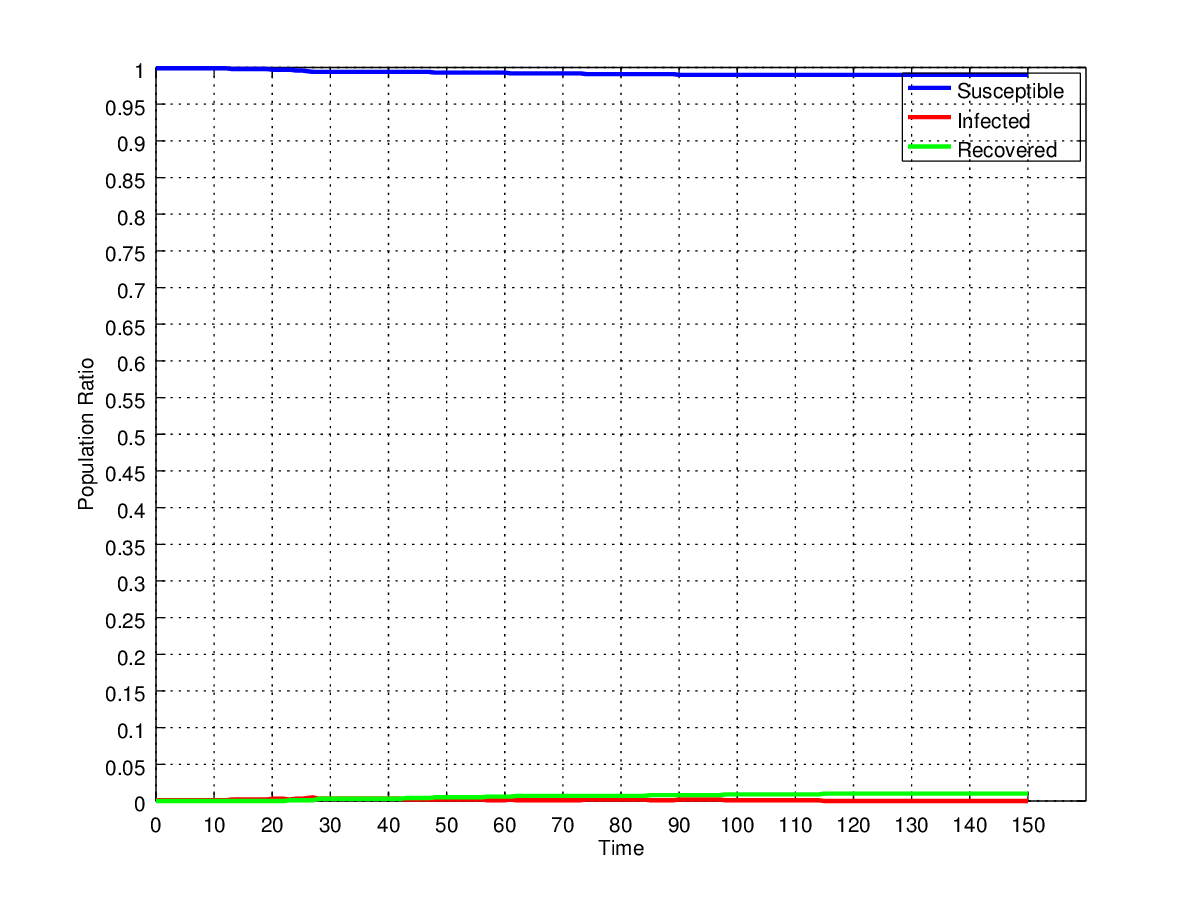
\includegraphics[width=1\textwidth, angle=0]{./../shared/fig/frabs/SIR_1000agents_150t_1dt_NOSS_parallel.png}
			\caption{$\Delta t = 1.0$}
			\label{fig:sir_abs_approximating_1dt}
		\end{subfigure}
    	&
		\begin{subfigure}[b]{0.3\textwidth}
			\centering
			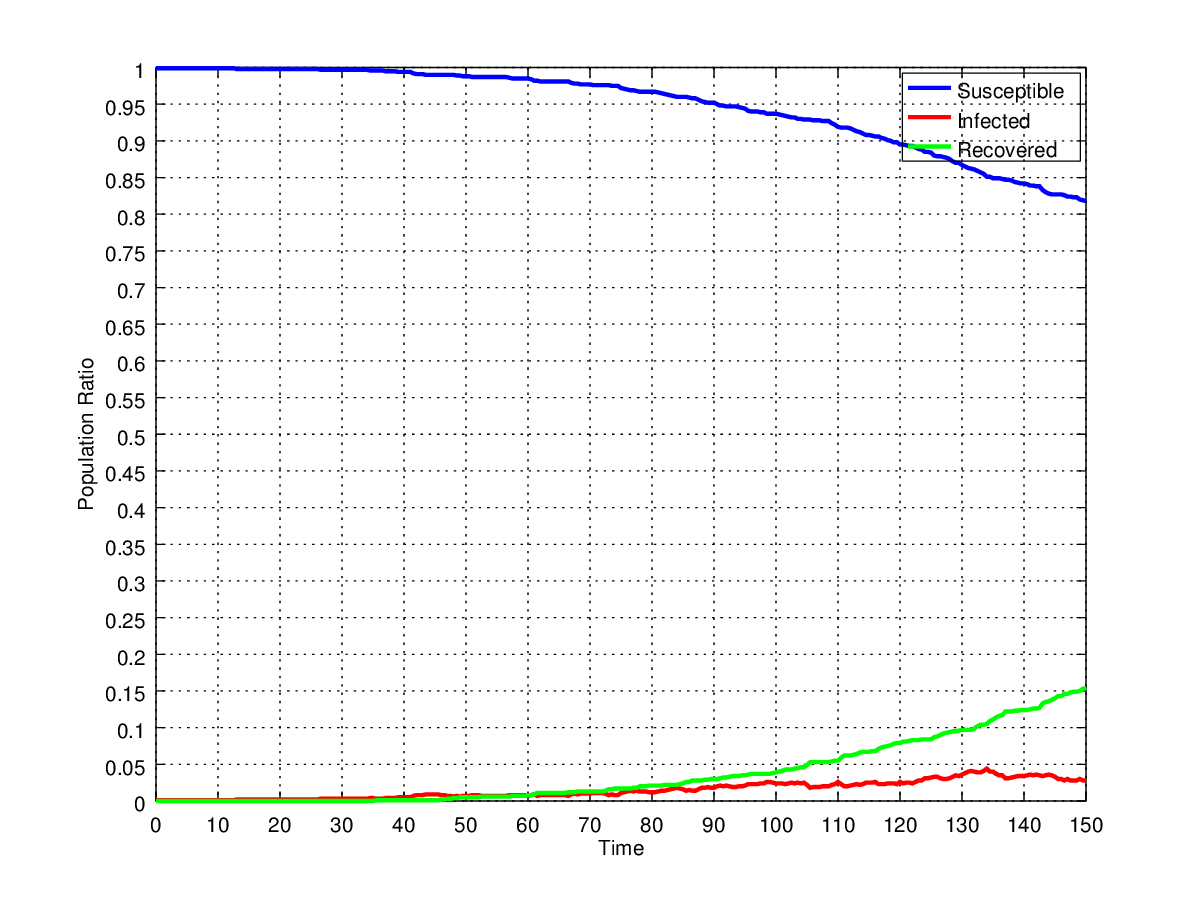
\includegraphics[width=1\textwidth, angle=0]{./../shared/fig/frabs/SIR_1000agents_150t_05dt_NOSS_parallel.png}
			\caption{$\Delta t = 0.5$}
			\label{fig:sir_abs_approximating_05dt}
		\end{subfigure}
    	
    	\\
    	
		\begin{subfigure}[b]{0.3\textwidth}
			\centering
			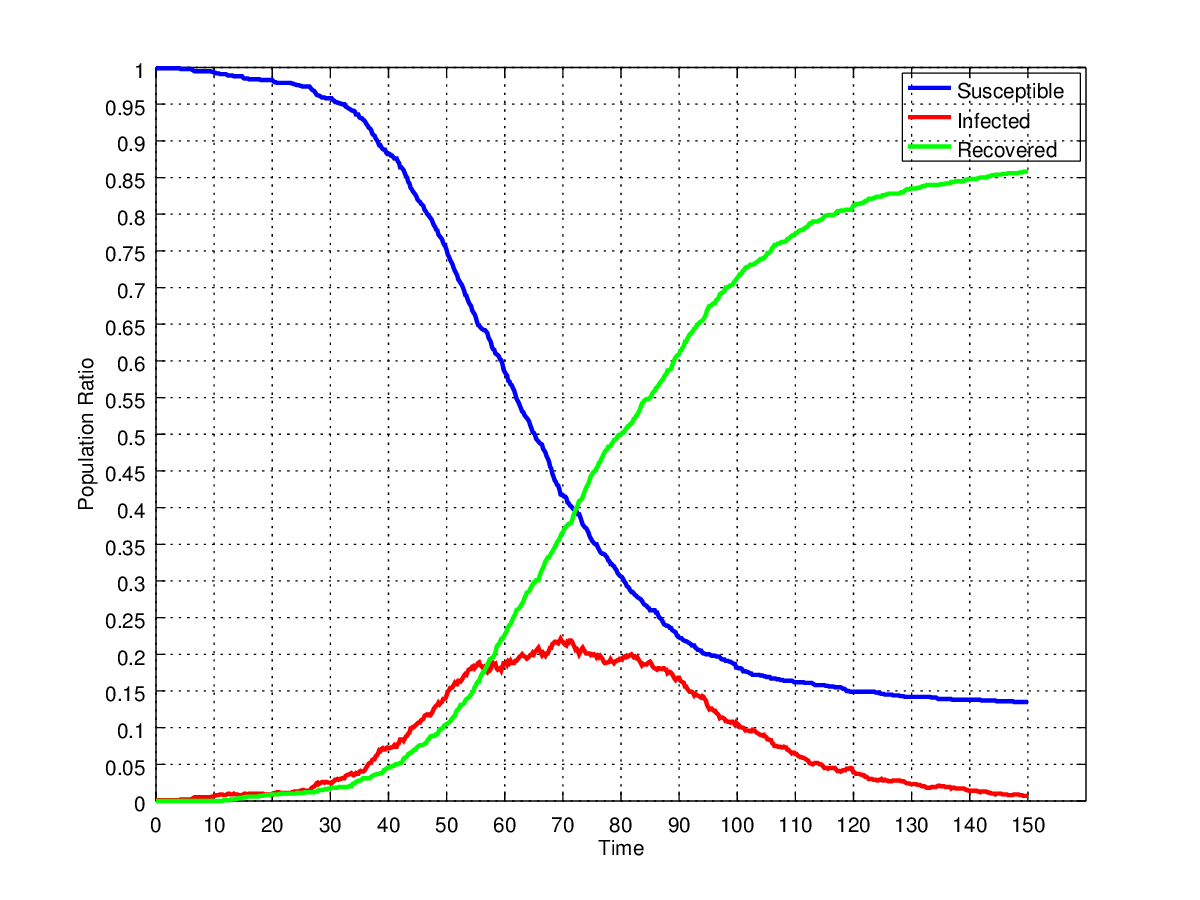
\includegraphics[width=1\textwidth, angle=0]{./../shared/fig/frabs/SIR_1000agents_150t_02dt_NOSS_parallel.png}
			\caption{$\Delta t = 0.2$}
			\label{fig:sir_abs_approximating_02dt}
		\end{subfigure}
		& 
		\begin{subfigure}[b]{0.3\textwidth}
			\centering
			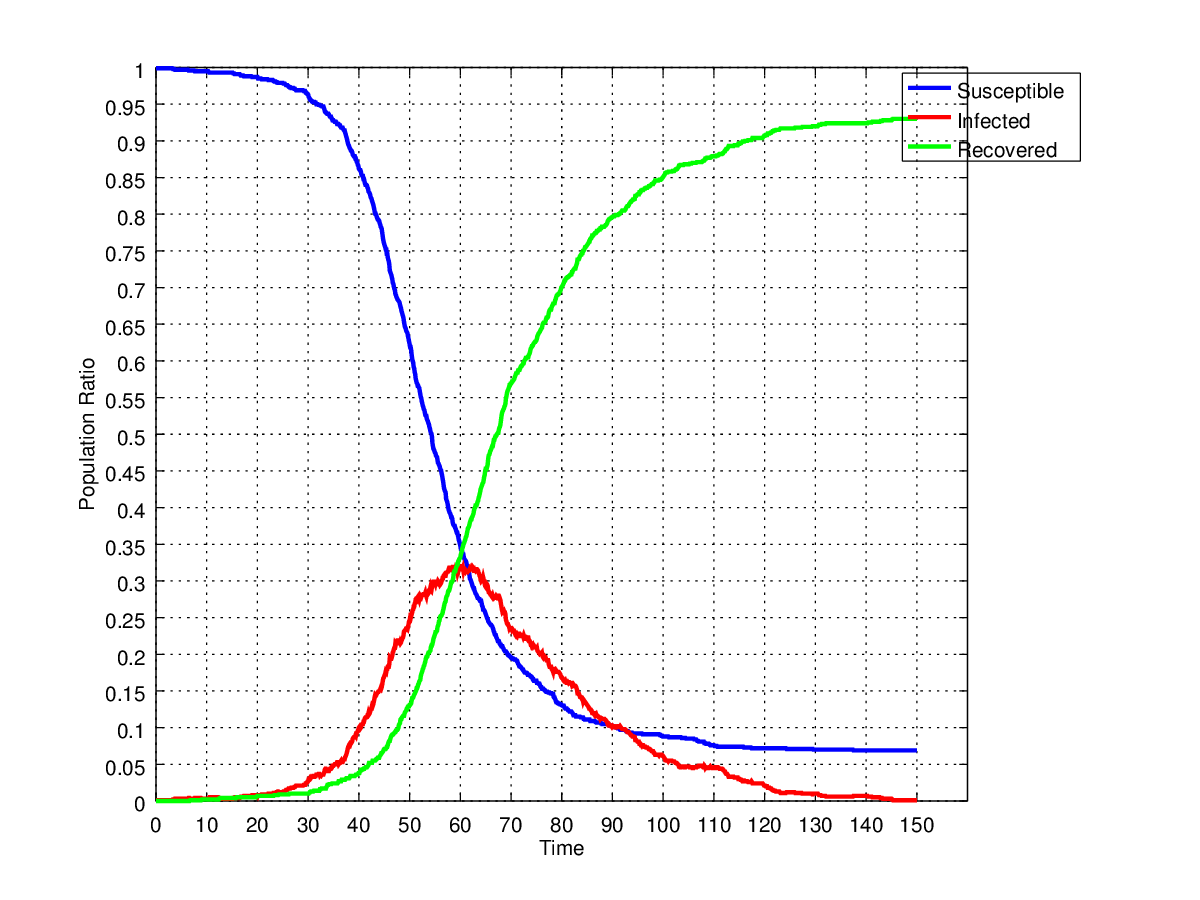
\includegraphics[width=1\textwidth, angle=0]{./../shared/fig/frabs/SIR_1000agents_150t_01dt_NOSS_parallel.png}
			\caption{$\Delta t = 0.1$}
			\label{fig:sir_abs_approximating_01dt}
		\end{subfigure}
	\end{tabular}
	
	\caption{Naive simulation of SIR using agent-based approach. Population Size $N$ = 1,000, contact rate $\beta = \frac{1}{5}$, infection probability $\gamma = 0.05$, illness duration $\delta = 15$ with initially 1 infected agent. Simulation run for 150 time-steps with various $\Delta t$.} 
	\label{fig:sir_abs_dynamics_naive}
\end{center}
\end{figure}

%TODO: reproducing about the same dynamics of the SD-solution (1.0 dt)
%	- super-sampling: 	contact-rate ss high, illness time-out low 
%	- agent number:		1000 vs. 10.000 agents
%	- Susceptibles making contact and infected response VS. only Infected make contact
%	- update-strat:		Sequential vs. Parallel
%	- making contact: susceptible only vs. susceptible AND infected
%	- do conversations make a difference?
%	- does a delayed switch (dSwitch) in transitions makes a difference?

Clearly something is going wrong as the dynamics do not resemble the ones of SD in any way with only 10 agents making the transition to infected to recovered. The problem is that we are running into sampling issues. TODO: explain deeper and better

\subsection{Sampling the System}
When sampling the system, the correct $\Delta t$ must be selected which depends on the highest frequency which occurs in a time-reactive function in the whole system. For example in the SIR model we want infected agents to make on average contact with $\beta = 5$ other agents per time-unit, which means with a frequency of $\frac{1}{5}$. This functionality is built on Yampas function \textit{occasionally} which behaviour we investigated under differing $\Delta t$ with the above frequency. In this investigation we simply sampled occasionally with different $\Delta t$ for a duration of $t = 1,000$ and the event-frequency of $\frac{1}{5}$. The result can be seen in Figure \ref{fig:sampling_occasionally_5evts} and is quite striking. The plot clearly shows that occasionally needs a quite high sampling frequency even for a comparatively low event-frequency, which becomes of course worse for higher event-frequencies.

The other time-reactive function which occurs in the SIR model is the timed transition from infected to recovered which occurs on average with an exponential random-distribution after $\delta = 15$. This functionality is built on a custom implementation of Yampas \textit{after} which creates an event after a time-out of the passed in time-duration drawn from an exponential random-distribution. Clearly this function has different semantics as although it also continuously emit events over time - \textit{NoEvent} before the time was hit, and \textit{Event b} after the time hit - the relevant point is that it switches to Event at some discrete point in time. This is implemented as simply adding up the $\Delta t$ until the accumulator is greater of equal than the previously drawn exponential time-out. We also investigated the behaviour of this function under varying $\Delta t$ using a time-out of $\delta = 15$. Our approach was to sample the \textit{afterExp} until an event occurs and then see when it has occurred. We run this with 10,000 replications with different random-number seeds and average the resulting times. The results can be seen in Figure \ref{fig:sampling_afterExp_5time}. The result is striking in another way: this function seems to be pretty invariant to the time-deltas, for obvious reasons: we are basically just interested in the "after"-condition of the whole semantics whereas in occasionally we are interested in the "repeatedly"-conditions. If we under-sample the \textit{afterExp} then we can be off by one $\Delta t$. If we under-sample \textit{occasionally} we keep loosing events - the less difference between $\Delta t$ and event-frequency, the more events we lose. Of course \textit{afterExp} can also be used for very short time-outs e.g. $\frac{1}{5}$. We have investigated the behaviour of this function for various $\Delta t$ as well as seen in Figure \ref{fig:sampling_afterExp_02time}. Here the result is much more striking and shows that \textit{afterExp} is vulnerable to small time-outs as well as \textit{occasionally}.  
To show that \textit{occasionally} is not vulnerable to very low frequencies of e.g. one event every 5 time-steps we plotted the behaviour of this under varying time-steps in Figure \ref{fig:sampling_occasionally_02evts}. The result shows that for low frequencies occasionally works fine with larger $\Delta t$.

\begin{figure}
\begin{center}
	\begin{tabular}{c c}
	\begin{subfigure}[b]{0.5\textwidth}
			\centering
			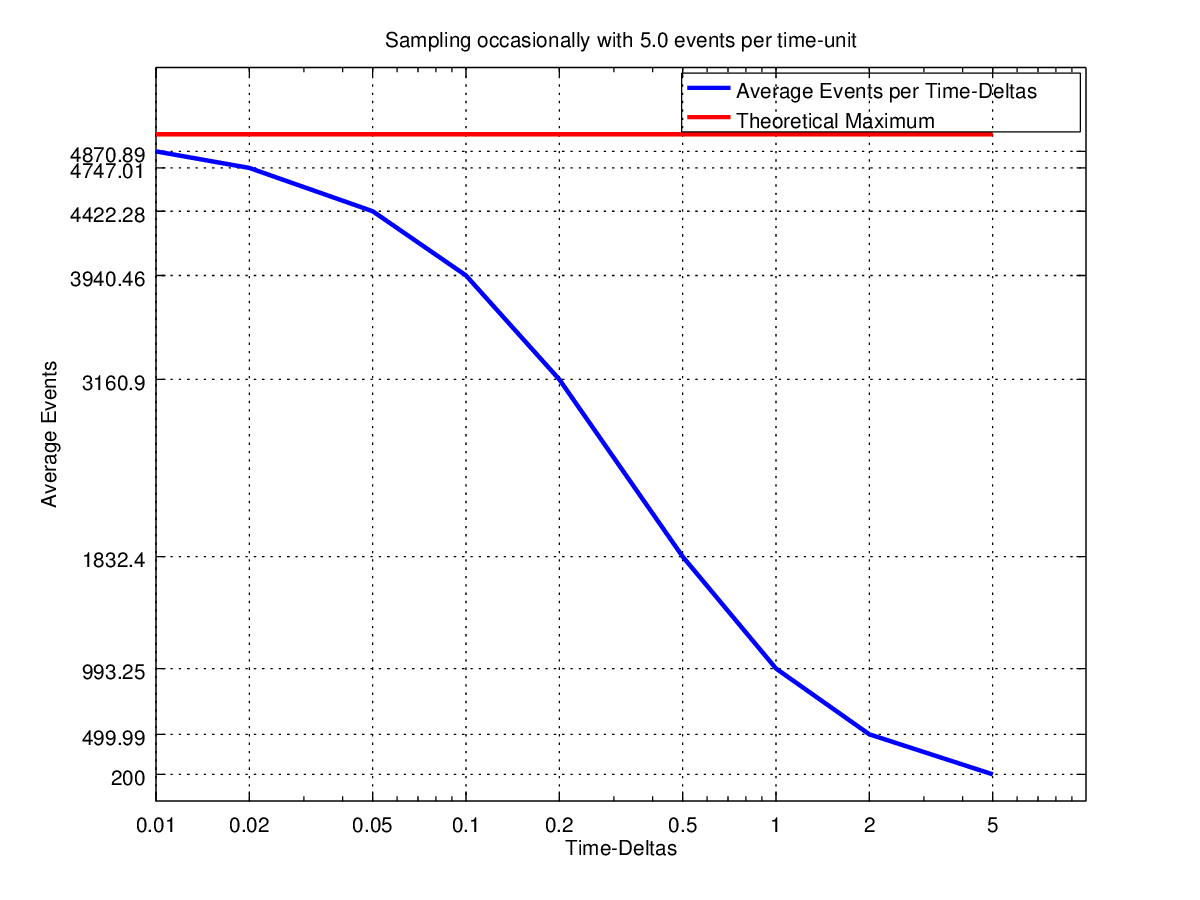
\includegraphics[width=.6\textwidth, angle=0]{./../shared/fig/sampling/samplingTest_occasionally_5evts.png}
			\caption{Sampling \textit{occasional} with a frequency of $\frac{1}{5}$ (average of 5 events per time-unit). The theoretical average is 5000 events within this time-frame.}
			\label{fig:sampling_occasionally_5evts}
		\end{subfigure}
		& 
		\begin{subfigure}[b]{0.5\textwidth}
			\centering
			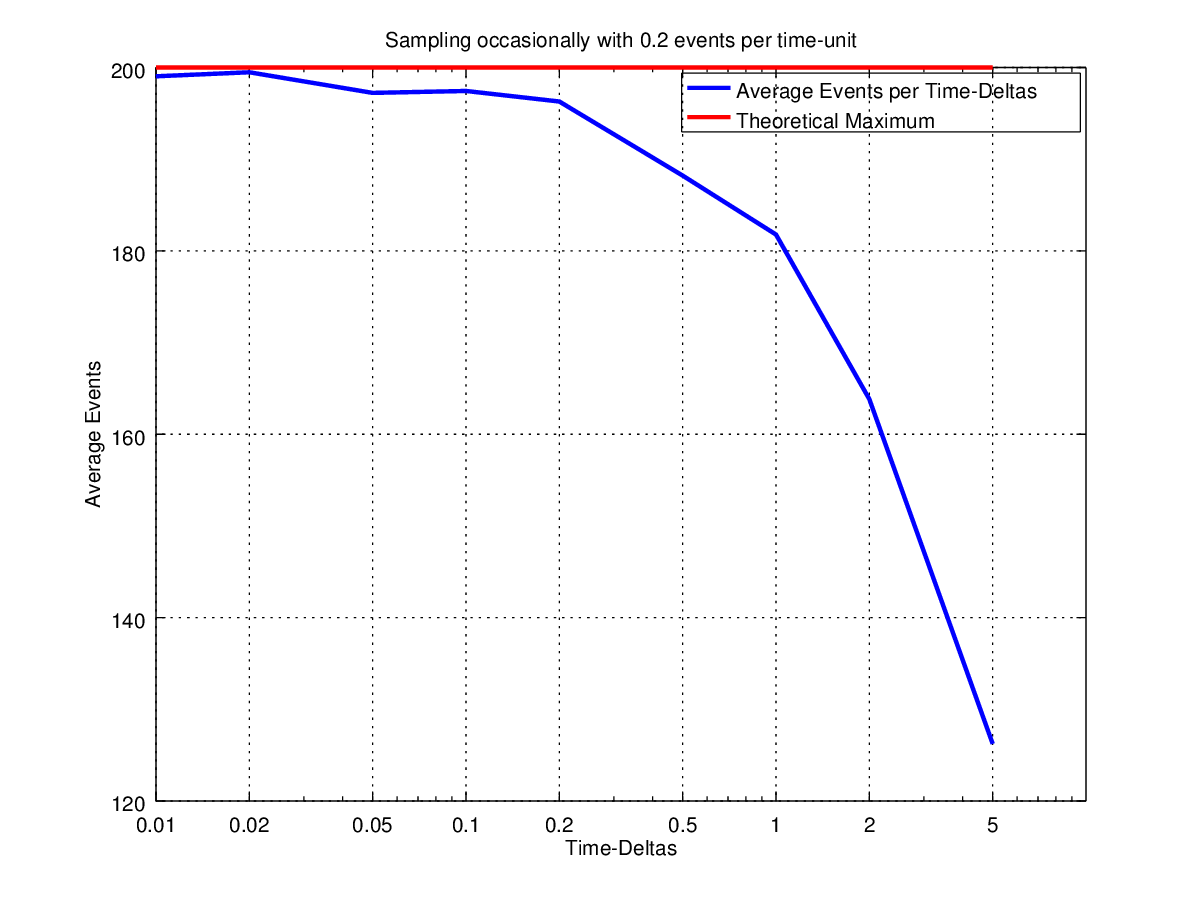
\includegraphics[width=.6\textwidth, angle=0]{./../shared/fig/sampling/samplingTest_occasionally_02evts.png}
			\caption{Sampling \textit{occasional} with a frequency of 5 (average of 0.2 events per time-unit). The theoretical average is 200 events within this time-frame.}
			\label{fig:sampling_occasionally_02evts}
		\end{subfigure}
		
		\\
		
		\begin{subfigure}[b]{0.5\textwidth}
			\centering
			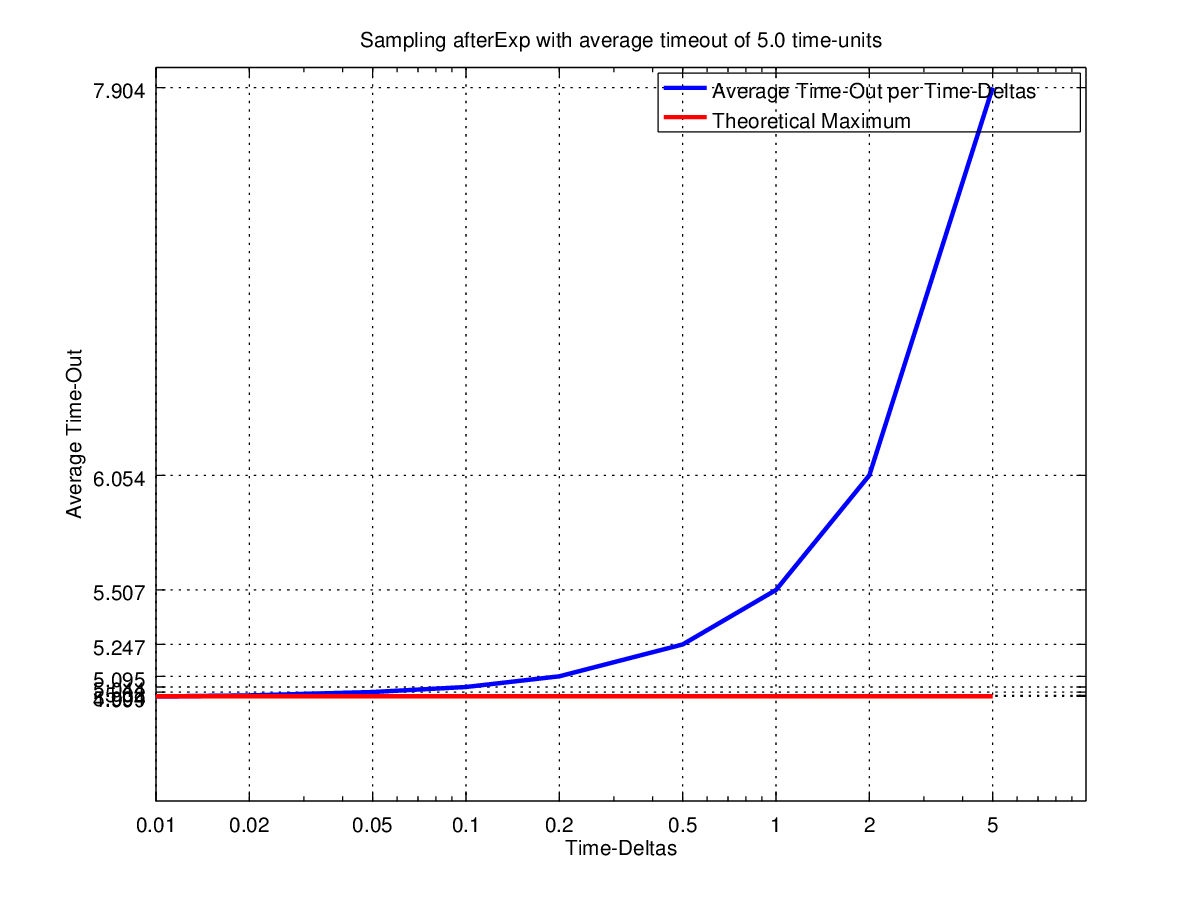
\includegraphics[width=.6\textwidth, angle=0]{./../shared/fig/sampling/samplingTest_afterExp_5time.png}
			\caption{Sampling \textit{afterExp} with an average time-out of 5.}
			\label{fig:sampling_afterExp_5time}
		\end{subfigure}
		& 
		\begin{subfigure}[b]{0.5\textwidth}
			\centering
			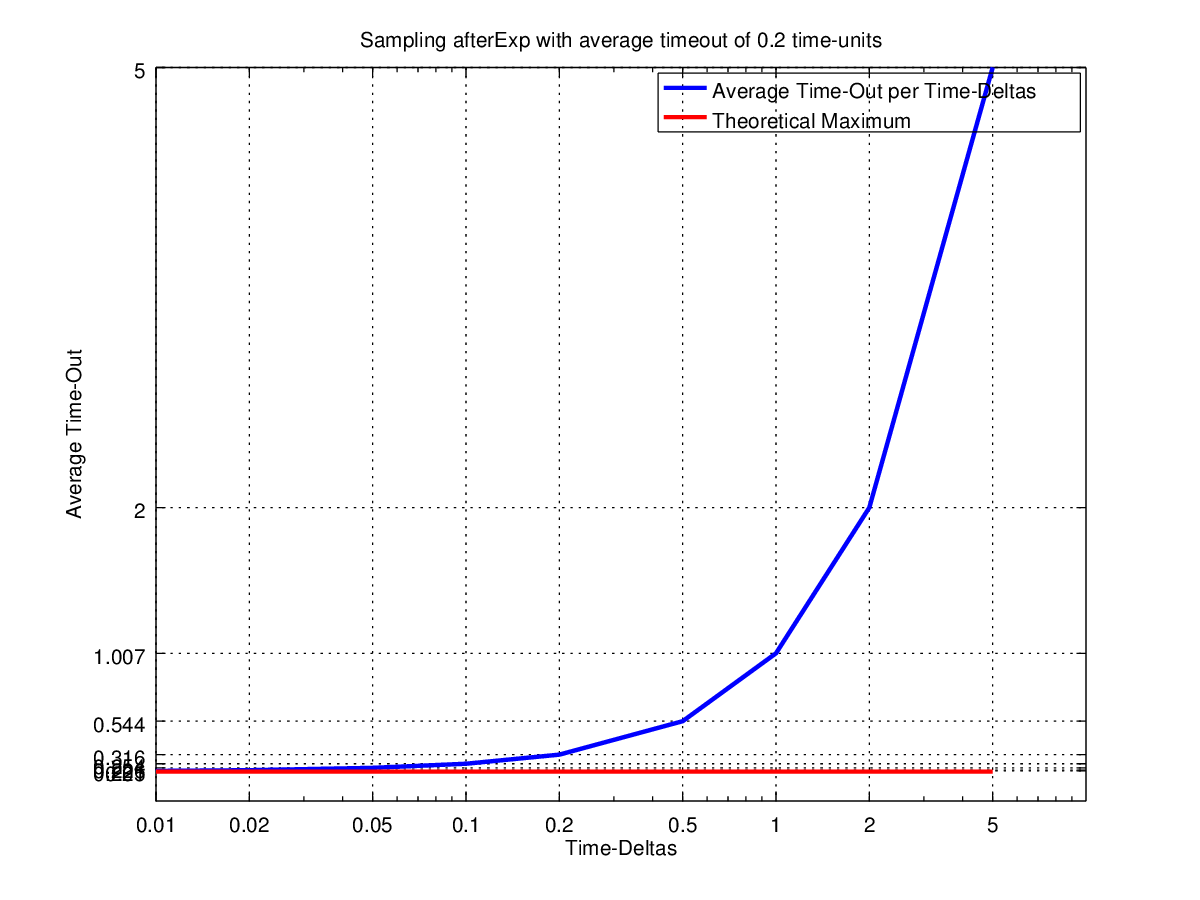
\includegraphics[width=.6\textwidth, angle=0]{./../shared/fig/sampling/samplingTest_afterExp_02time.png}
			\caption{Sampling \textit{afterExp} with an average time-out of 0.2.}
			\label{fig:sampling_afterExp_02time}
		\end{subfigure}
	\end{tabular}
	
	\caption{Sampling the \textit{afterExp} and \textit{occasional} functions to visualise the influence of sampling frequencies on the occurrence of the respective events. $\Delta t$ are [ 5, 2, 1, $\frac{1}{2}$, $\frac{1}{5}$, $\frac{1}{10}$, $\frac{1}{20}$, $\frac{1}{50}$, $\frac{1}{100}$ ]. The experiments for \textit{afterExp} used 10,000 replications. The experiments for \textit{occasional} ran for $t= 1,000$ with 100 replications.} 
	\label{fig:sampling_tests}
\end{center}
\end{figure}

\subsection{Increasing the frequency}
Using these observation we run simulations with varying $\Delta t$ with $\Delta = 0.5$, $\Delta = 0.2$ and $\Delta = 0.1$ with the results visible in Figures \ref{fig:sir_abs_approximating_05dt}, \ref{fig:sir_abs_approximating_02dt} and \ref{fig:sir_abs_approximating_01dt} but still when decreasing $\Delta t$ we don't approach the SD dynamics. As previously mentioned the agent-based approach is a discrete one which means that with increasing number of agents, the discrete dynamics approximate the continuous dynamics of the SD simulation. We run further simulations with $\Delta = 0.1$ but with varying agent numbers to see the influence with the results seen in Figure \ref{fig:sir_abs_approximating}.

\begin{figure}
\begin{center}
	\begin{tabular}{c c}
		\begin{subfigure}[b]{0.3\textwidth}
			\centering
			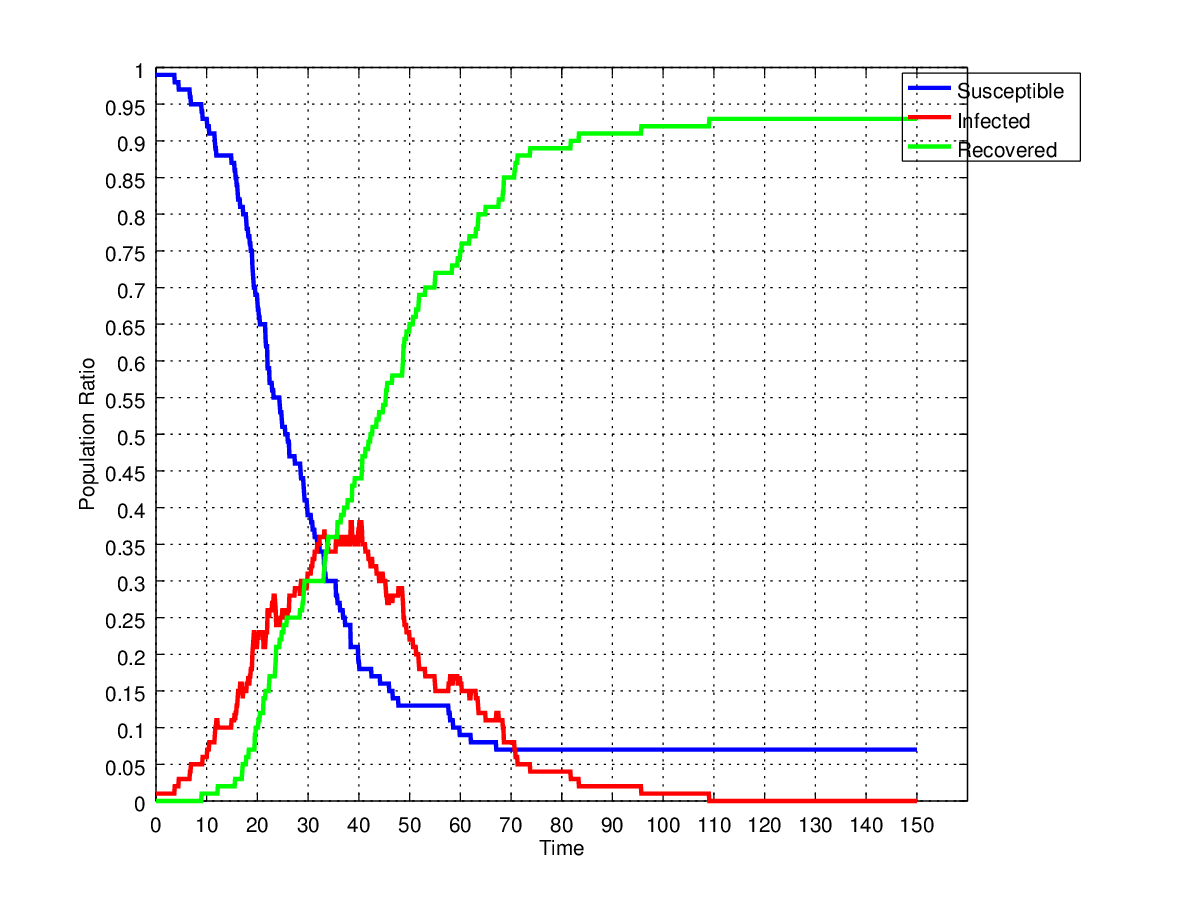
\includegraphics[width=1\textwidth, angle=0]{./../shared/fig/frabs/SIR_100agents_150t_01dt_NOSS_parallel.png}
			\caption{100 Agents}
			\label{fig:sir_abs_approximating_100}
		\end{subfigure}
    	&
		\begin{subfigure}[b]{0.3\textwidth}
			\centering
			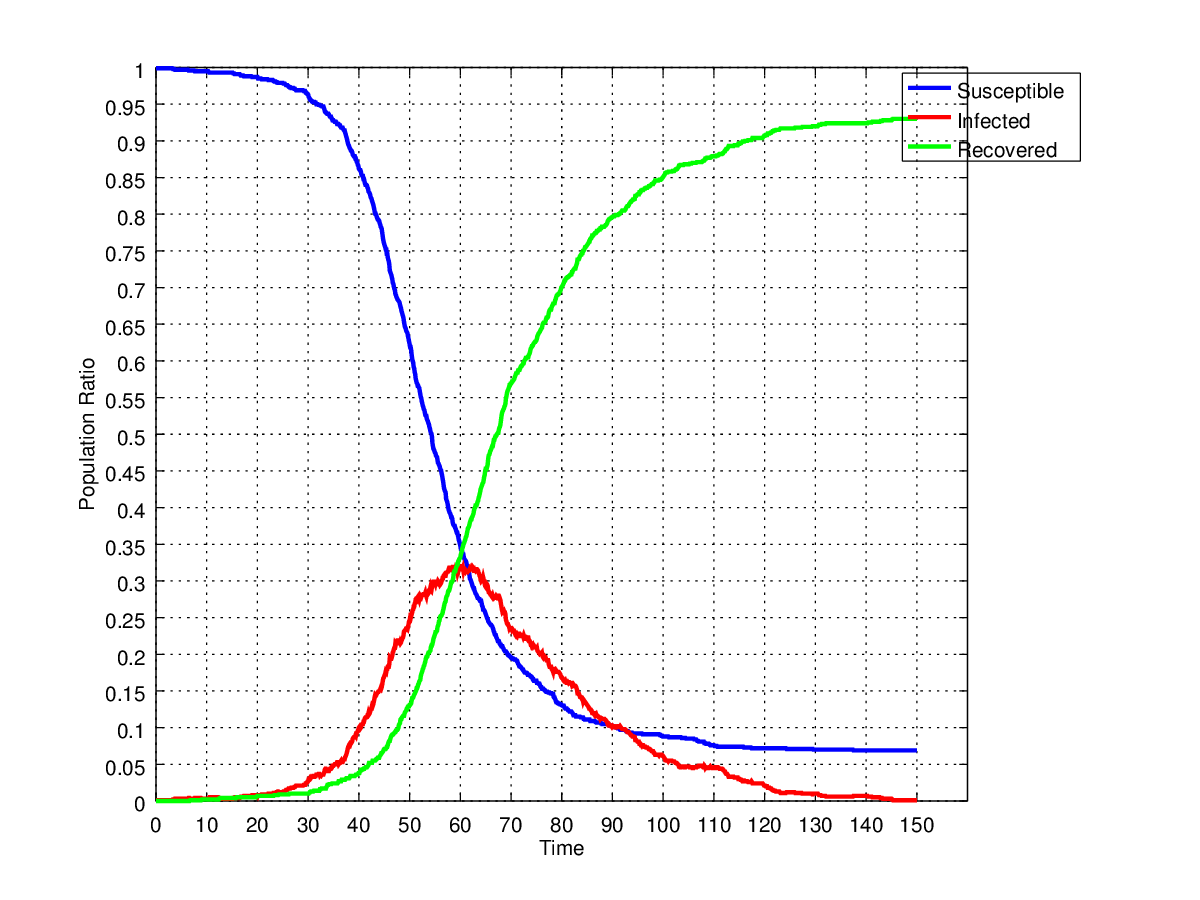
\includegraphics[width=1\textwidth, angle=0]{./../shared/fig/frabs/SIR_1000agents_150t_01dt_NOSS_parallel.png}
			\caption{1,000 Agents}
			\label{fig:sir_abs_approximating_1000}
		\end{subfigure}
    	
    	\\
    	
		\begin{subfigure}[b]{0.3\textwidth}
			\centering
			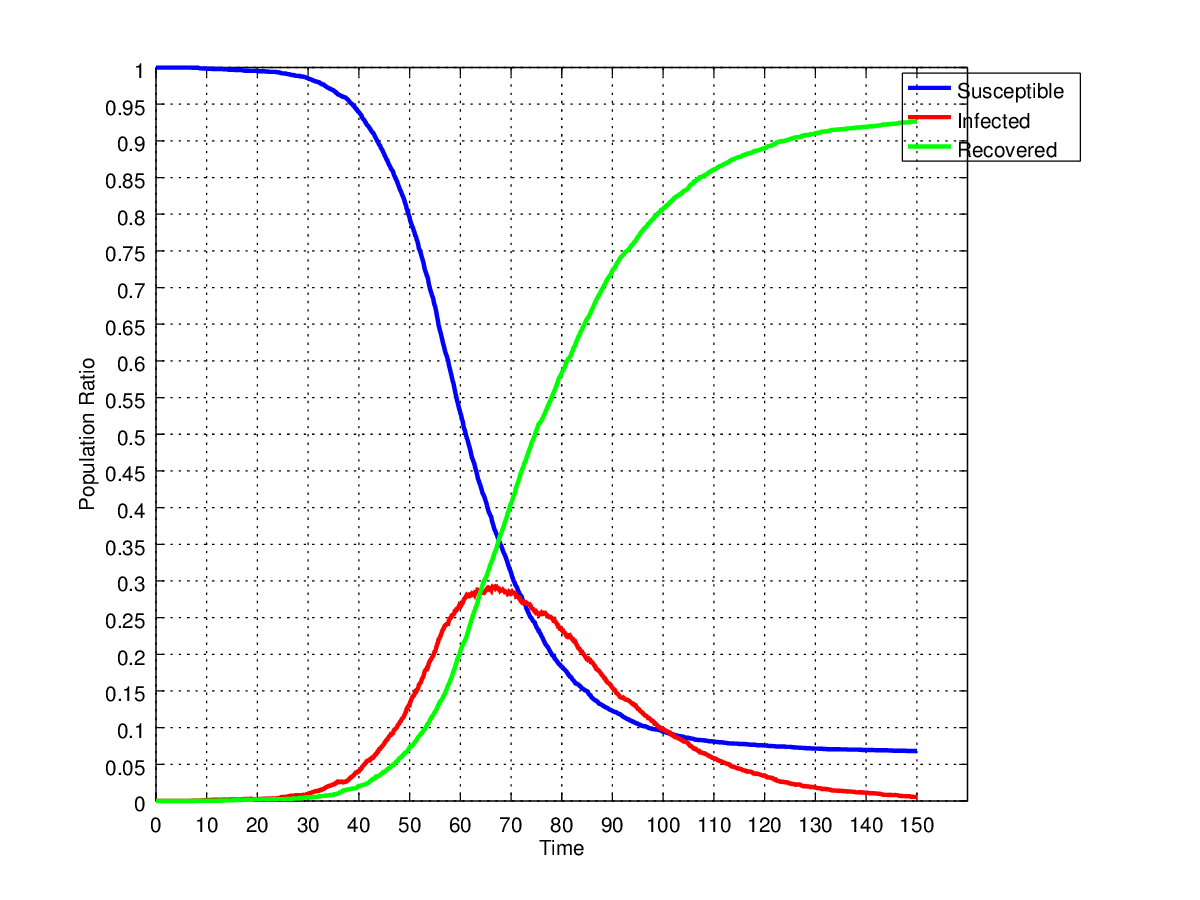
\includegraphics[width=1\textwidth, angle=0]{./../shared/fig/frabs/SIR_5000agents_150t_01dt_NOSS_parallel.png}
			\caption{5,000 Agents}
			\label{fig:sir_abs_approximating_5000}
		\end{subfigure}
		& 
		\begin{subfigure}[b]{0.3\textwidth}
			\centering
			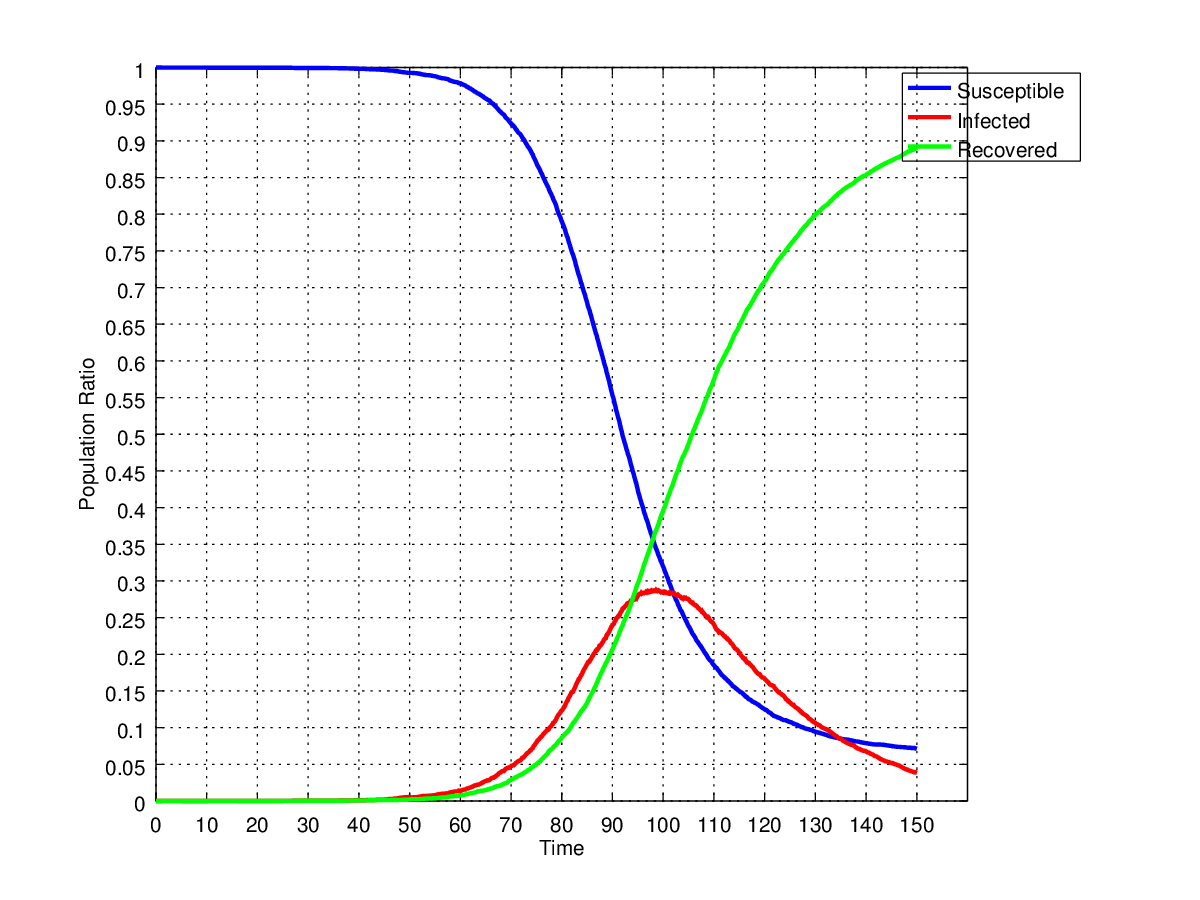
\includegraphics[width=1\textwidth, angle=0]{./../shared/fig/frabs/SIR_10000agents_150t_01dt_NOSS_parallel.png}
			\caption{10,000 Agents}
			\label{fig:sir_abs_approximating_10000}
		\end{subfigure}
	\end{tabular}
	
	\caption{Varying agent numbers with same model-parameters except population size. All simulations run for 150 time-steps with $\Delta t = 0.1$}
	\label{fig:sir_abs_approximating}
\end{center}
\end{figure}

Although increasing the number of agents improves our approximation, still the dynamics of 10,000 Agents are still nowhere close to the SD dynamics. This is because as opposed to SD, which is deterministic, the agent-based approach is inherently a stochastic one as we continuously draw from random-distributions which drive our state-transitions. What we see in Figure \ref{fig:sir_abs_approximating} is then just a single run where the dynamics would result in slightly different shapes when run with a different random-number generator seed. The agent-based approach thus generates a distribution of dynamics over which ones needs to average to arrive at the correct solution. 

\subsection{Adding replications}
To average over multiple runs with different random-number seeds one uses replications in which the simulation is run with the exact same parameters multiple times but each with a different random-number generator seed. The resulting dynamics are then averaged which will result in much smother results.
We have done this in Figure \ref{fig:sir_abs_agents_repls}, using 10 replications. The results are not yet matching the SD dynamics completely but we have increased our approximation considerably. Note that in the replications we are using 10 initially infected agents to ensure that no simulation run will terminate too early. An early termination means that the disease gets extinct after a few time steps which would offset the dynamics completely. This happens due to "unlucky" random distributions which can be repaired by introducing more initially infected agents which increases the probability of spreading the disease in the very early stage of the simulation drastically. We found that when using 10 initially infected agents in a population of thousands is enough to never result in an early terminating simulation. In the case of 100 agents, 10 initially infected ones might be too much and distorts the dynamics but this is irrelevant in this case. This is also a fundamental difference between SD and ABS: the dynamics of the agent-based approach can result in a wide range of scenarios which includes also the one in which the disease gets extinct in the early stages - a lucky coincidence for mankind. Though this is simply not possible in the SD approach because as soon as there are more than 0 infected agents at the start of the simulation, the dynamics will take off. Thus we argue that ABS is much closer to reality than SD as it allows to explore alternate futures in the dynamics.

\begin{figure}
\begin{center}
	\begin{tabular}{c c}
		\begin{subfigure}[b]{0.3\textwidth}
			\centering
			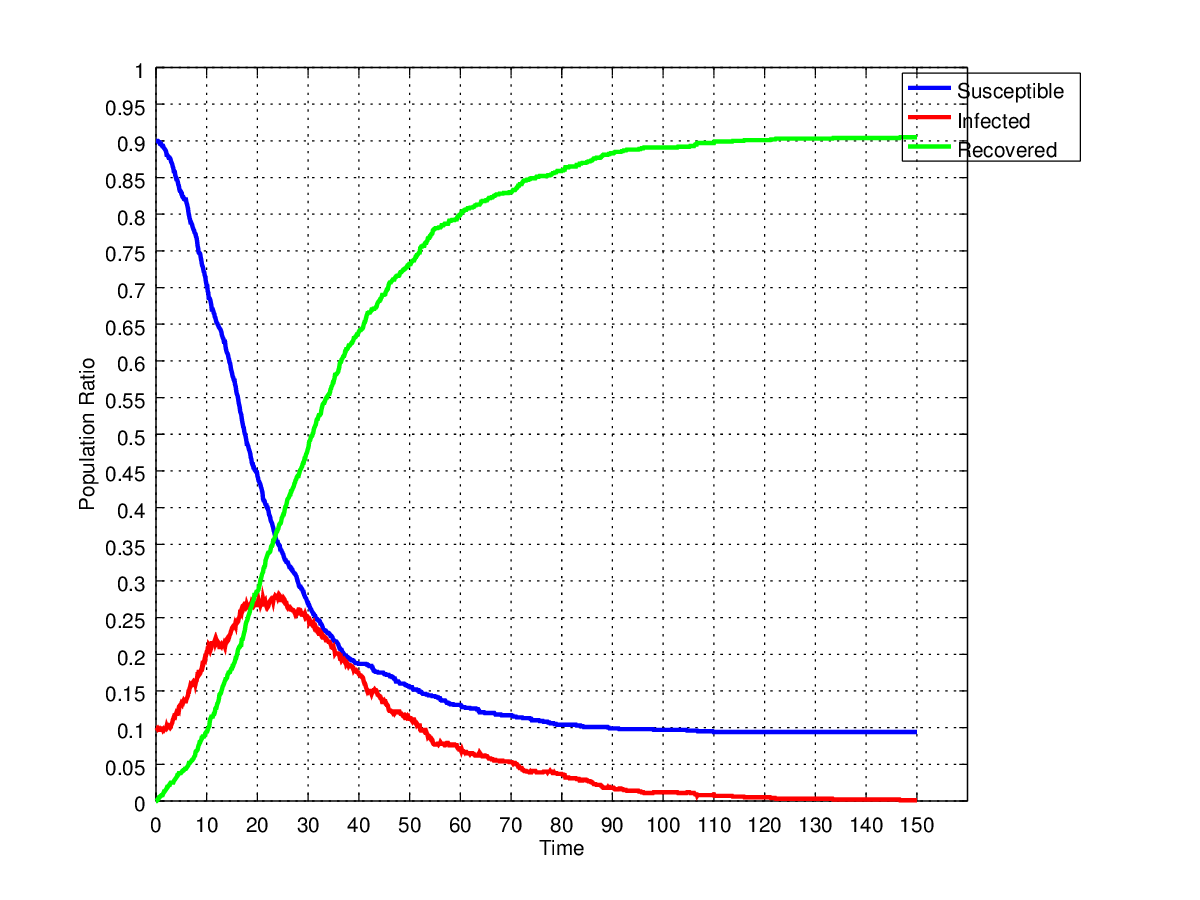
\includegraphics[width=1\textwidth, angle=0]{./../shared/fig/frabs/SIR_100agents_150t_01dt_NOSS_parallel_10replications.png}
			\caption{100 Agents}
			\label{fig:sir_abs_agents_repls_100}
		\end{subfigure}
    	&
		\begin{subfigure}[b]{0.3\textwidth}
			\centering
			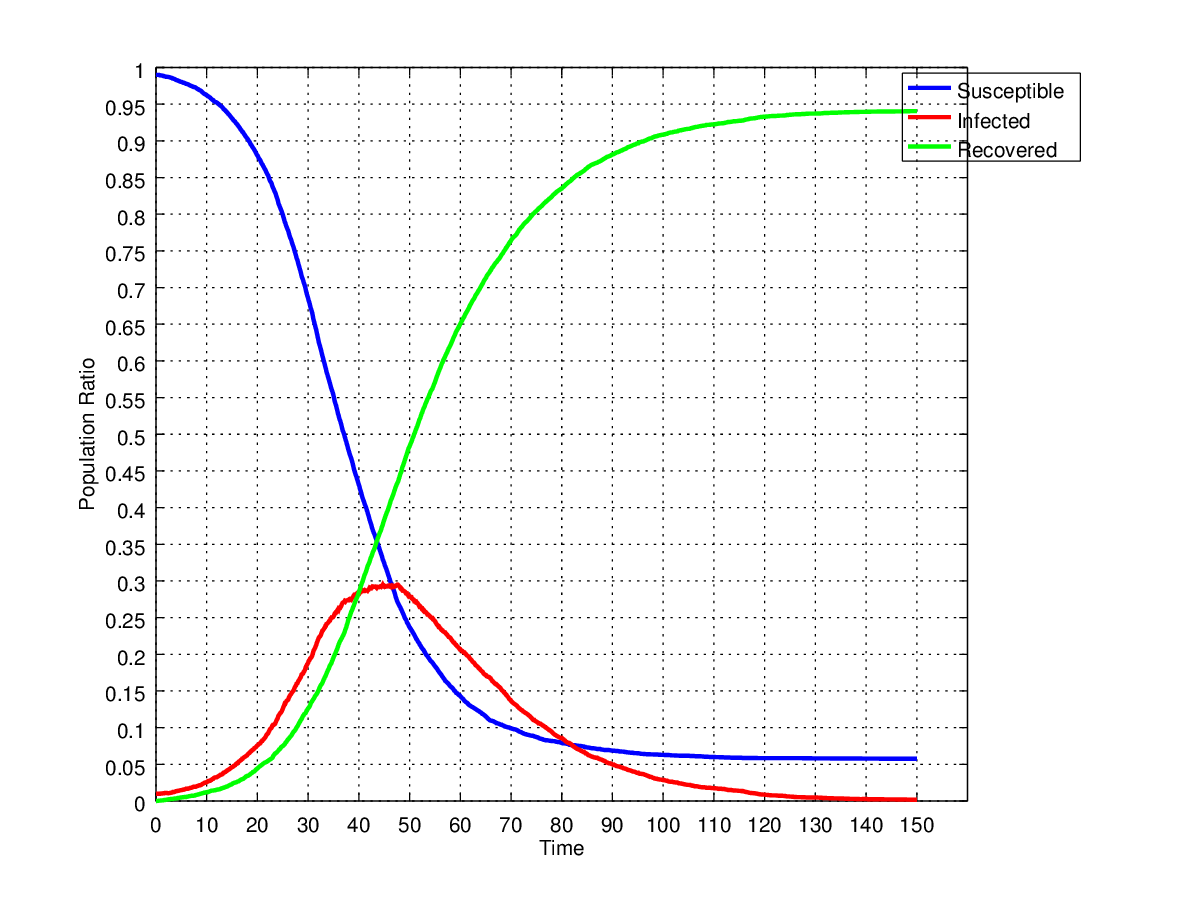
\includegraphics[width=1\textwidth, angle=0]{./../shared/fig/frabs/SIR_1000agents_150t_01dt_NOSS_parallel_10replications.png}
			\caption{1,000 Agents}
			\label{fig:sir_abs_agents_repls_1000}
		\end{subfigure}
    	
    	\\
    	
		\begin{subfigure}[b]{0.3\textwidth}
			\centering
			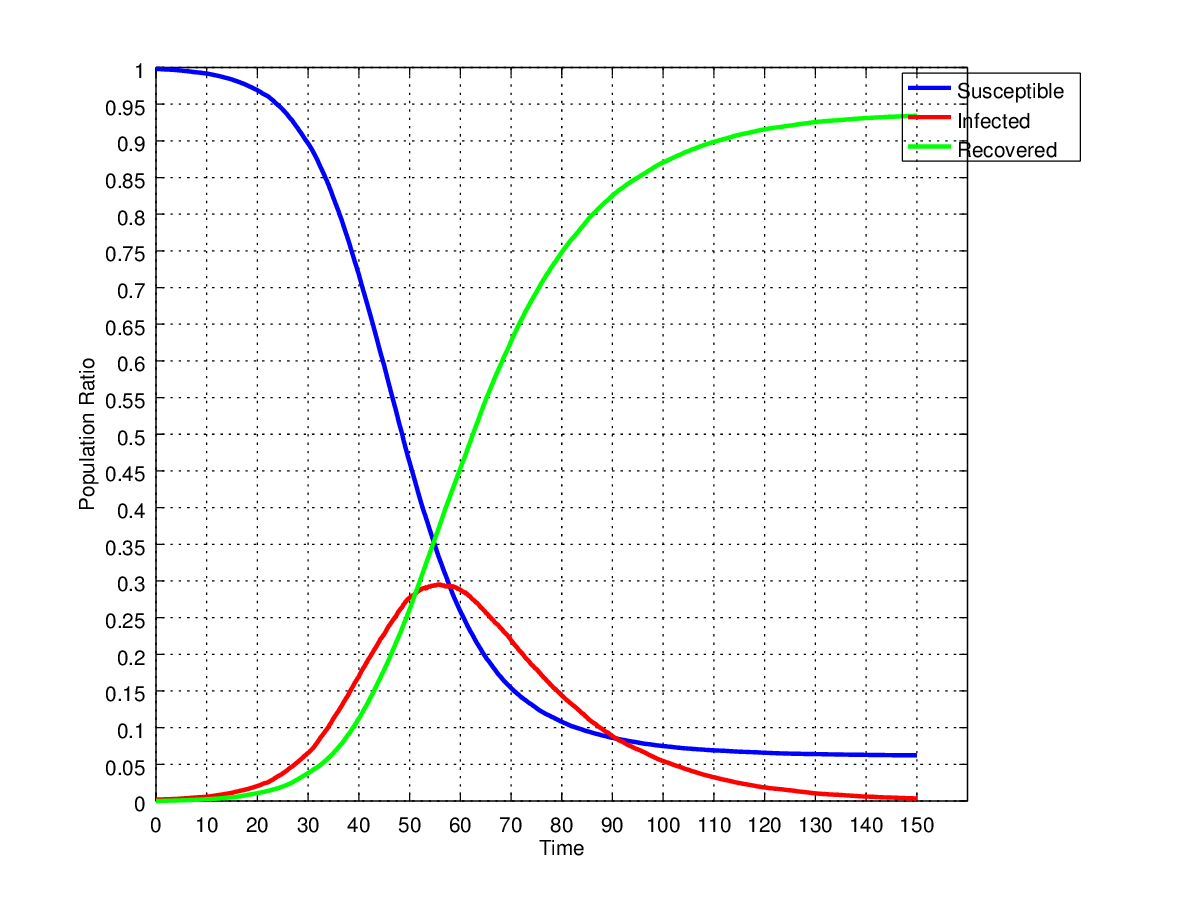
\includegraphics[width=1\textwidth, angle=0]{./../shared/fig/frabs/SIR_5000agents_150t_01dt_NOSS_parallel_10replications.png}
			\caption{5,000 Agents}
			\label{fig:sir_abs_agents_repls_5000}
		\end{subfigure}
		&
		\begin{subfigure}[b]{0.3\textwidth}
			\centering
			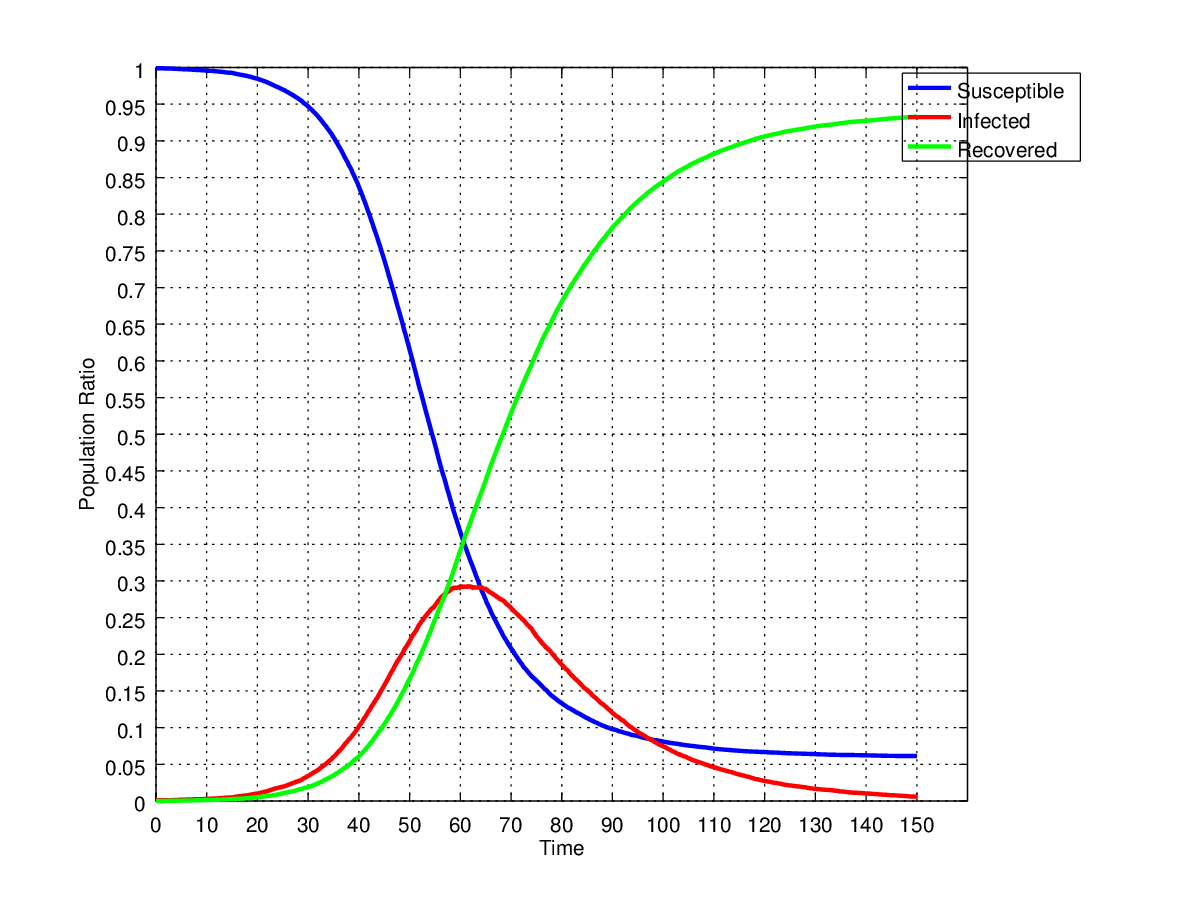
\includegraphics[width=1\textwidth, angle=0]{./../shared/fig/frabs/SIR_10000agents_150t_01dt_NOSS_parallel_4replications.png}
			\caption{10,000 Agents}
			\label{fig:sir_abs_agents_repls_10000}
		\end{subfigure}
	\end{tabular}
	
	\caption{Dynamics of Figure \ref{fig:sir_abs_approximating} averaged over 10 replications with initially 10 infected agents.} 
	\label{fig:sir_abs_agents_repls}
\end{center}
\end{figure}

%When comparing the results of the dynamics of the agent-based approach from Figure \ref{fig:sir_abs_approximating} and Figure \ref{fig:sir_abs_agents_repls} to the SD dynamics of Figure \ref{fig:sir_sd_dynamics} it becomes apparent that by increasing the number of agents the dynamics approximate the SD dynamics with increasing accuracy. Still although using 5,000 agents and replications seem to be not enough yet, we need to increase our number of agents to 10,000

Still although using a quite small $\Delta t = 0.1$ and using replications we are not yet approximating the SD dynamics to a satisfactory level. The only option we have is to further decrease $\Delta t$. Of course performance is a big issue and it decreases as $\Delta t$ get smaller and smaller. This is because when running a simulation for a duration of $t$ and sampling it with $\Delta t$ then the steps to calculate is $\frac{t}{\Delta t}$. In each step all agents are run, messages delivered and environments folded and updated which implies that the more steps the lower the performance. The problem is that not the whole system needs to run on a very high frequency, only the corresponding functions which need to be sampled at high frequency. If we could perform super-sampling just for the given high-frequency functions with the whole system running in lower frequency then we could achieve a substantial performance boost and make it feasible to sample parts at much higher frequencies.

\subsection{Adding Super-Sampling}
In Yampa there exists a function \textit{embed} which allows to run a given signal-function with provided $\Delta t$ but the problem is that this function does not really help because it does not return a signal-function. What we need is a signal-function which takes the number of super-samples \textit{n}, the signal-function \textit{sf} to sample and returns a new signal-function which performs super-sampling on it:

\begin{minted}[fontsize=\footnotesize]{haskell}
superSampling :: Int -> SF a b -> SF a [b]
\end{minted}

It does this by evaluating \textit{sf} for \textit{n} times, each with $\Delta t = \frac{\Delta t}{n}$ and the same input argument \textit{a} for all \textit{n} evaluations. At time 0 no super-sampling is done and just a single output of \textit{sf} is calculated. A list of \textit{b} is returned with length of \textit{n} containing the result of the \textit{n} evaluations of \textit{sf}. If 0 or less super samples are requested exactly one is calculated.

We ran tests super-sampling both \textit{occasionally} Figure \ref{fig:sampling_occasionally_ss_02evts}, Figure \ref{fig:sampling_occasionally_ss_5evts} and \textit{afterExp} Figure \ref{fig:sampling_afterExp_ss_5time}, Figure \ref{fig:sampling_afterExp_ss_02time}. They work the same way as above except that now $\Delta t = 1.0$ but using increasing numbers of super-samples. The results are as expected: as the number of super-samples increase, so increases the accuracy.

\begin{figure*}
\begin{center}
	\begin{tabular}{c c}
		\begin{subfigure}[b]{0.5\textwidth}
			\centering
			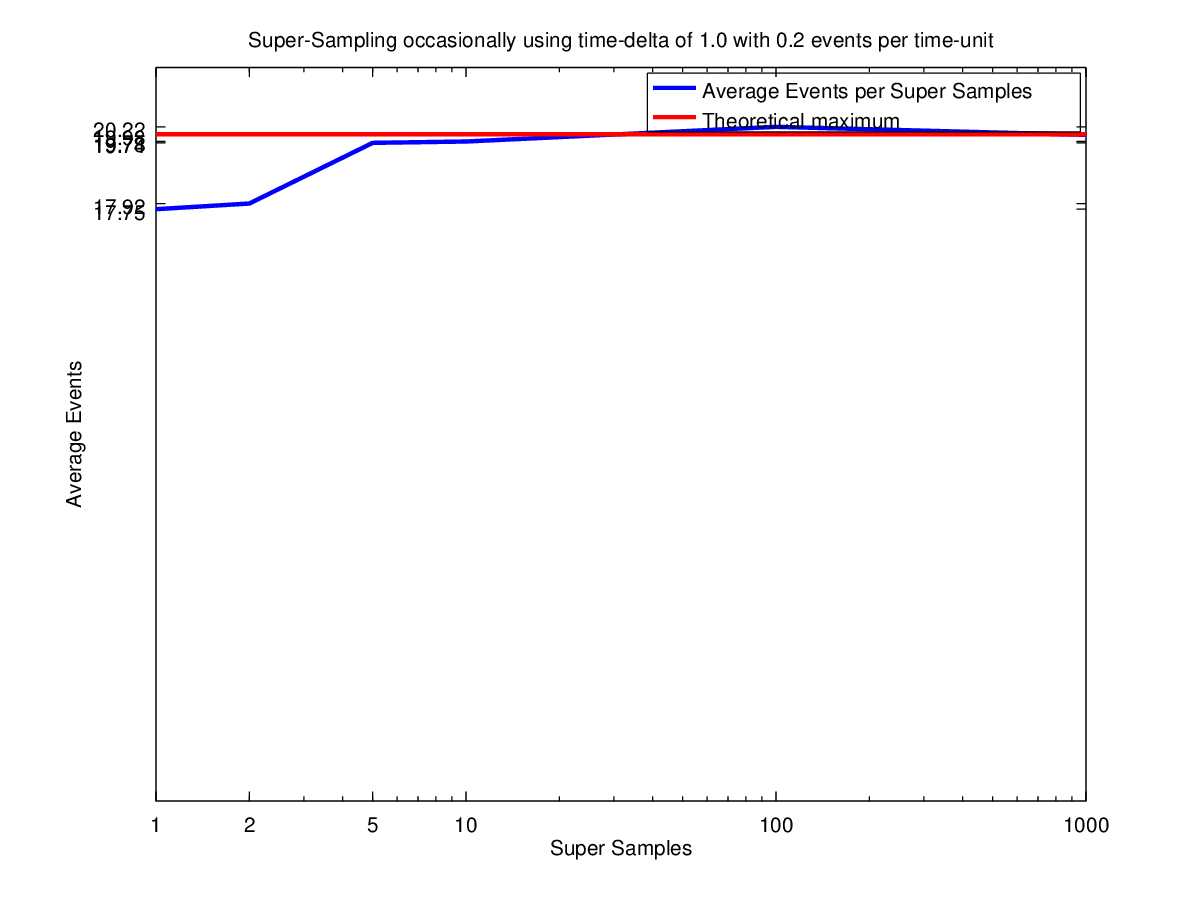
\includegraphics[width=.6\textwidth, angle=0]{./../shared/fig/sampling/samplingTest_occasionally_ss_02evts.png}
			\caption{Super-Sampling the \textit{occasional} function with event-frequency of 5 (average of 0.2 events per time-unit). The theoretical average is 20 event within this time-frame.}
			\label{fig:sampling_occasionally_ss_02evts}
		\end{subfigure}
		&
		\begin{subfigure}[b]{0.5\textwidth}
			\centering
			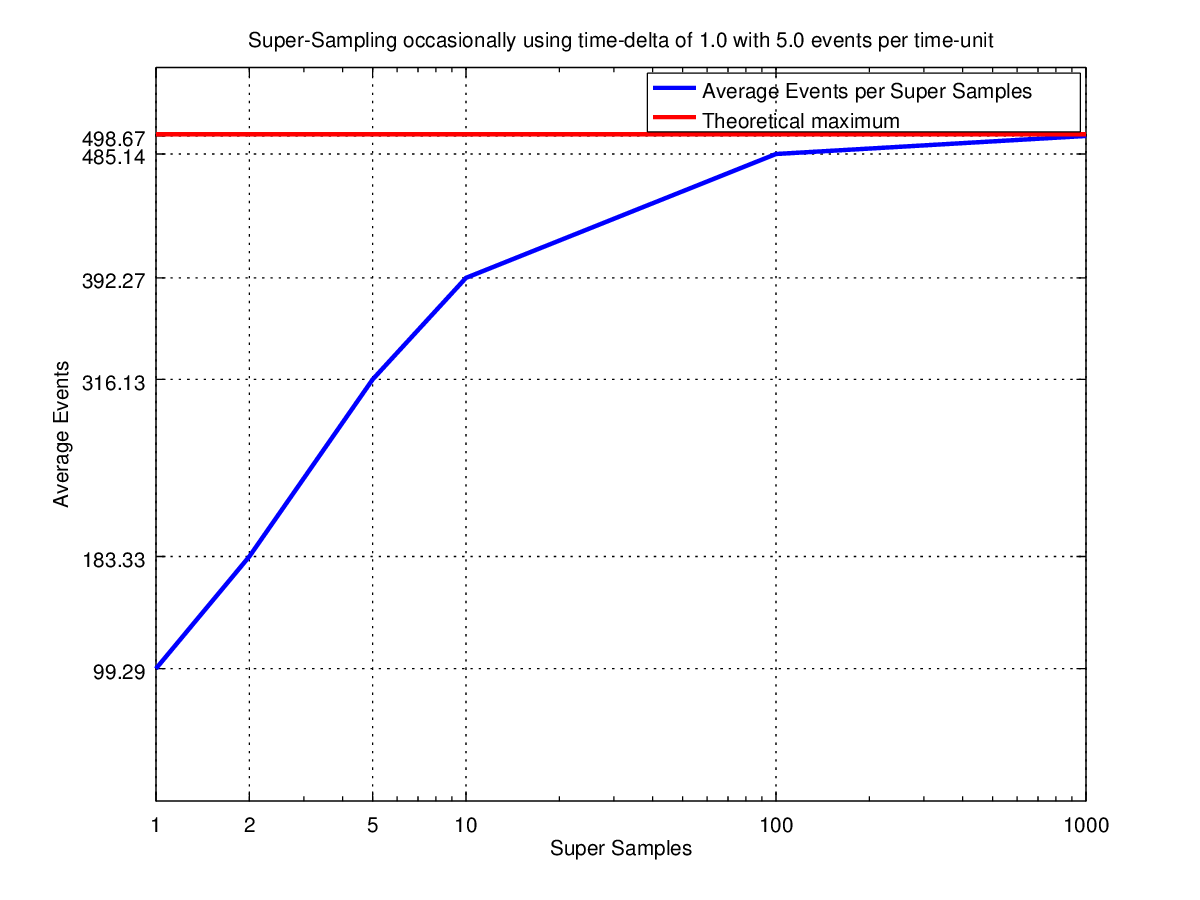
\includegraphics[width=.6\textwidth, angle=0]{./../shared/fig/sampling/samplingTest_occasionally_ss_5evts.png}
			\caption{Super-Sampling the \textit{occasional} function with event-frequency of $\frac{1}{5}$ (average of 5 events per time-unit). The theoretical average is 500 event within this time-frame.}
			\label{fig:sampling_occasionally_ss_5evts}
		\end{subfigure}

		\\
		
		\begin{subfigure}[b]{0.5\textwidth}
			\centering
			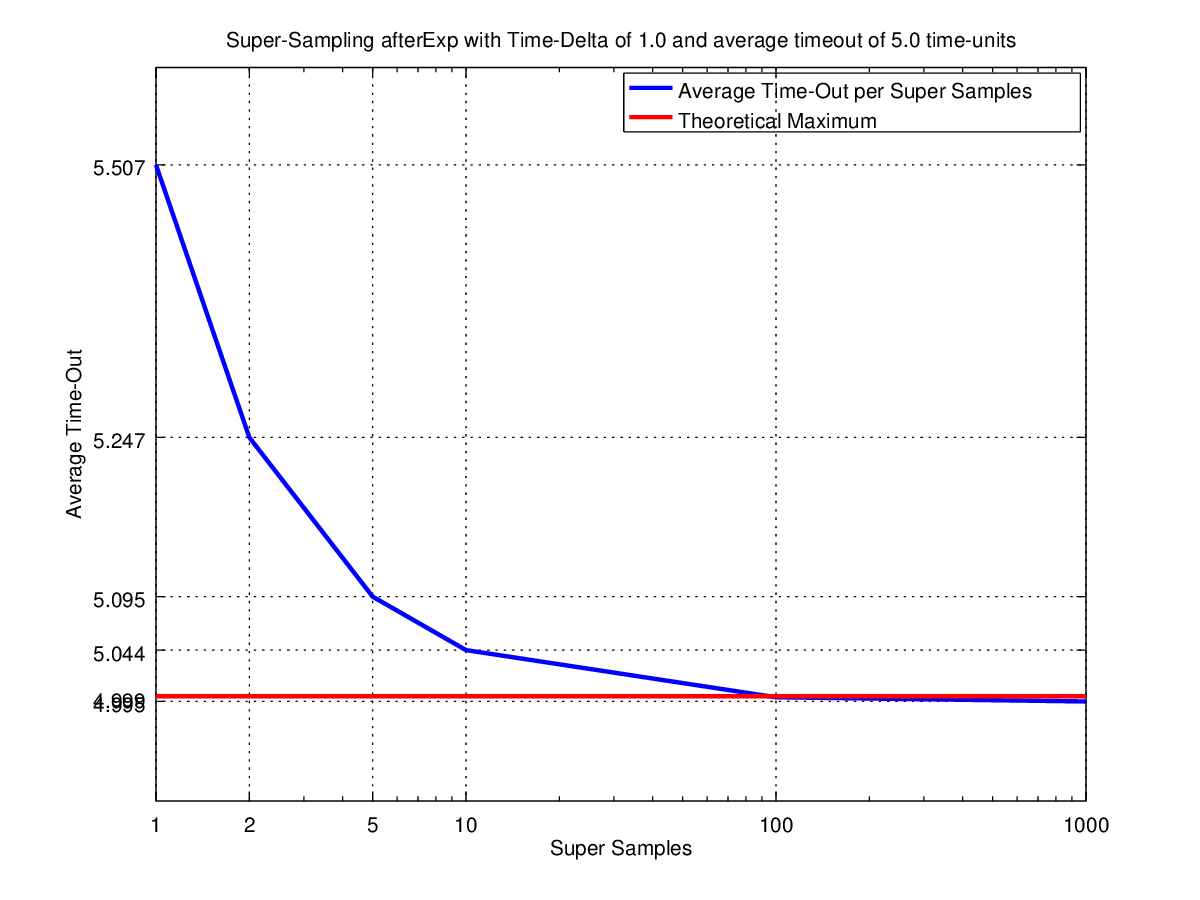
\includegraphics[width=.6\textwidth, angle=0]{./../shared/fig/sampling/samplingTest_afterExp_SS_5time.png}
			\caption{Super-Sampling the \textit{afterExp} function with average time-out of 5.}
			\label{fig:sampling_afterExp_ss_5time}
		\end{subfigure}
		&
		\begin{subfigure}[b]{0.5\textwidth}
			\centering
			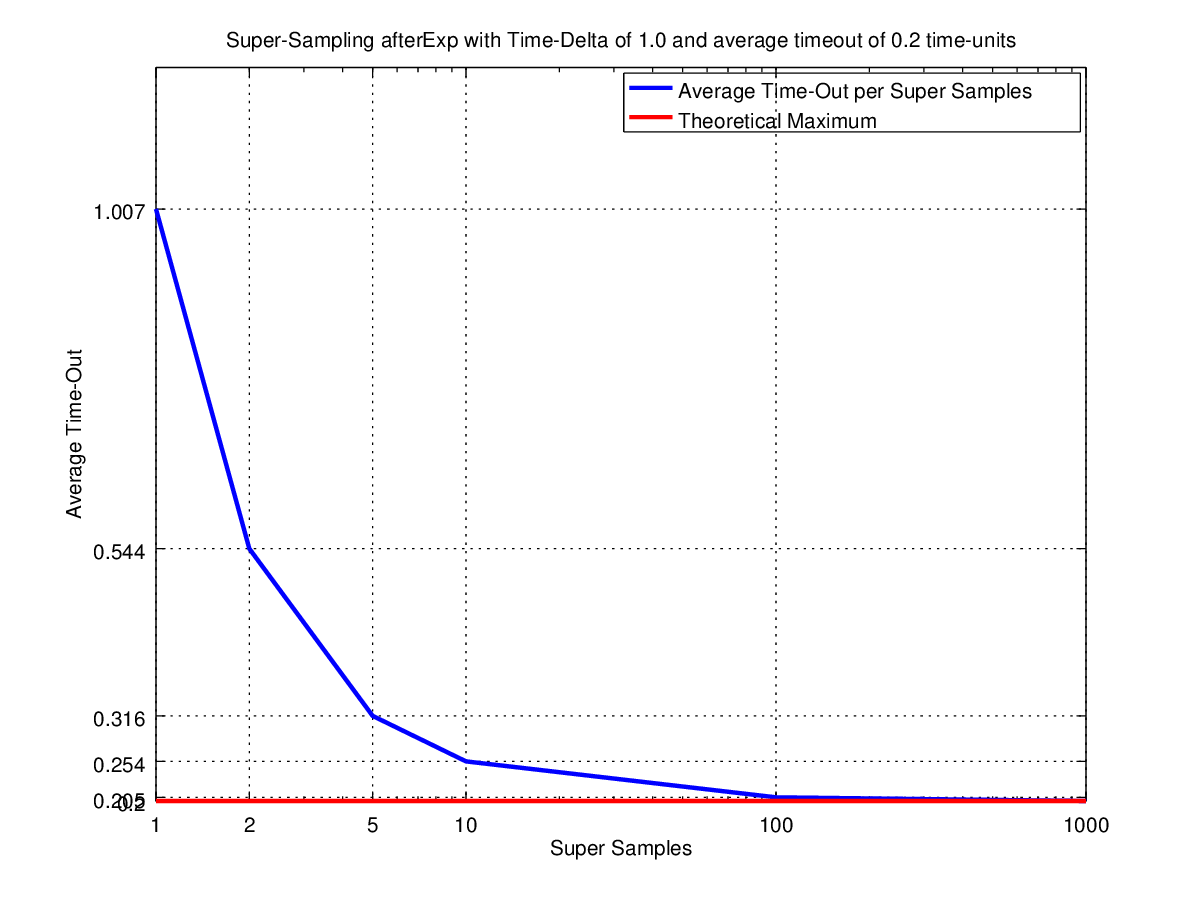
\includegraphics[width=.6\textwidth, angle=0]{./../shared/fig/sampling/samplingTest_afterExp_SS_02time.png}
			\caption{Super-Sampling the \textit{afterExp} function with average time-out of 0.2.}
			\label{fig:sampling_afterExp_ss_02time}
		\end{subfigure}
	\end{tabular}
	
	\caption{Super-Sampling the \textit{afterExp} and \textit{occasional} functions to visualize the influence of increasing number of super-samples on the average occurrence of the respective events. The $\Delta t = 1.0$ in both cases with super-samples of [1, 2, 5, 10, 100, 1000]. The experiments for \textit{afterExp} used 10,000 replications. The experiments for \textit{occasional} ran for $t = 100$ with 100 replications.} 
	\label{fig:supersampling_tests}
\end{center}
\end{figure*}

At first this might not seem to be a real win as we still need to calculate a big number of samples every time. The big win comes though when these super-sampled signal-functions are embedded in a larger system which could run on a comparatively low frequency of $\Delta t = 1.0$. So we are then increasing the sampling-frequency just where we need it and keep the frequency low where it is not required.

We are using super-sampling in our SIR implementation to increase performance. We do this by setting $\Delta t = 1.0$ and super-sampling the relevant functions with time-semantics which are \textit{transitionAfterExp} and \textit{sendMessageOccationallySrc}. For both we provide in our EDSL versions which support super-sampling:

\begin{minted}[fontsize=\footnotesize]{haskell}
sendMessageOccasionallySrcSS :: RandomGen g => g -> Double -> Int -> MessageSource 
                                -> SF (AgentOut, e) AgentOut
                                
transitionAfterExpSS :: RandomGen g => g -> Double -> Int 
                        -> AgentBehaviour -> AgentBehaviour -> AgentBehaviour
\end{minted}

Both now take an additional parameter which determines the number of super-samples to be calculated. According to the above observations of the \textit{occasionally} and \textit{afterExp} functions which are the foundations of both of the functions we sample \textit{sendMessageOccasionallySrcSS} with 20 super-samples and \textit{transitionAfterExpSS} with 2. This will ensure that by using $\Delta t = 1.0$ we only calculate $t$ steps when running a simulation for $t$ time but that we sample our relevant functions with enough resolution to capture its frequencies. Optimally we should increase the number of super-samples for \textit{sendMessageOccasionallySrcSS} to about 100. This will result in lower performance as \textit{every} agent will perform this super-sampling. So in the end it is a struggle of performance vs. sufficiently close approximation. We define the number of super-samples in lines 29 and 32 and use the functions in line 95 and 104 of Appendix \ref{app:abs_code}.

\subsection{The final detail: messaging delay}
Unfortunately when setting $\Delta t = 1.0$ the dynamics of the agent-based approach won't approach the dynamics of the SD, despite using super-sampling as can be seen in Figure \ref{fig:sir_10000_1dt}.

\begin{figure}
\begin{center}
	\begin{tabular}{c c}
		\begin{subfigure}[b]{0.5\textwidth}
			\centering
			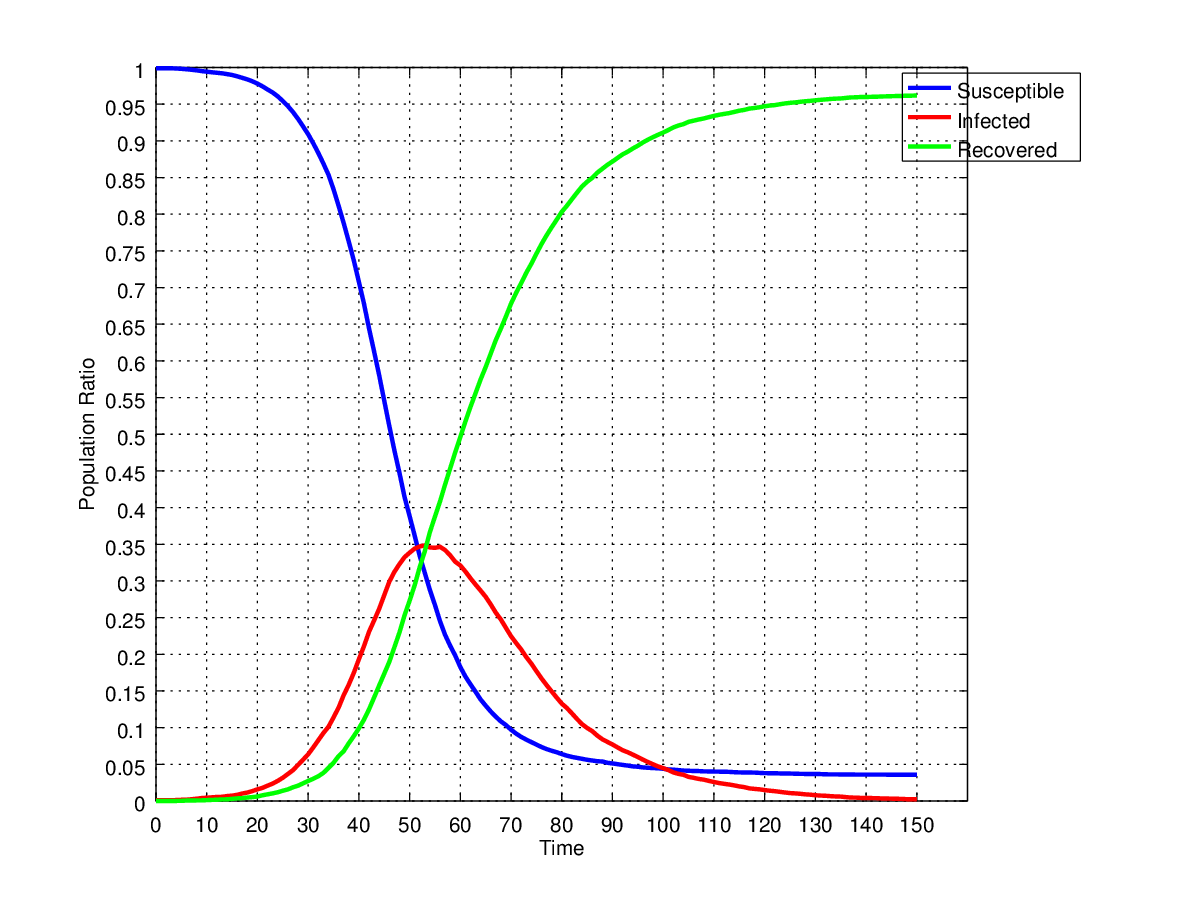
\includegraphics[width=.8\textwidth, angle=0]{./../shared/fig/frabs/SIR_10000agents_150t_1dt_parallel.png}
			\caption{$\Delta t = 1.0$}
			\label{fig:sir_10000_1dt}
		\end{subfigure}
	
		&
		
		\begin{subfigure}[b]{0.5\textwidth}
			\centering
			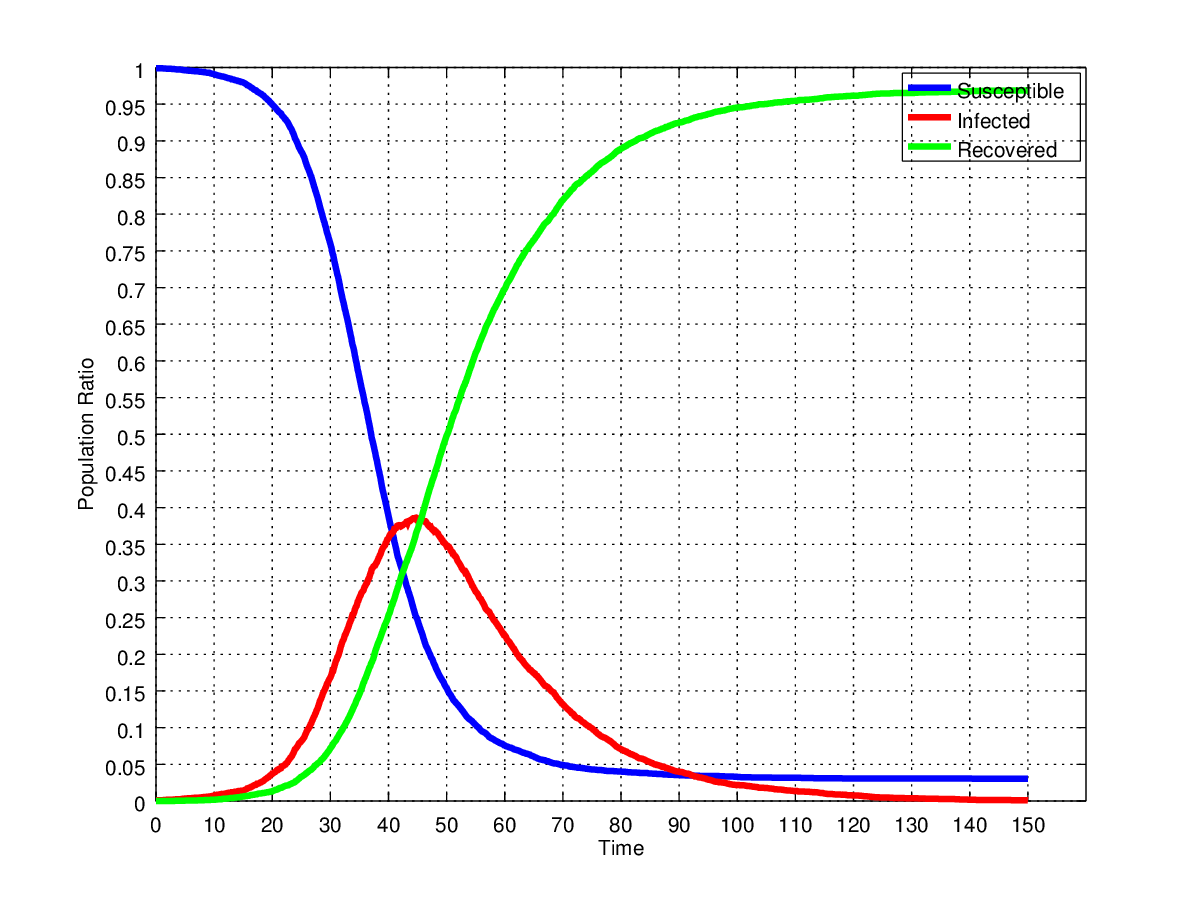
\includegraphics[width=.8\textwidth, angle=0]{./../shared/fig/frabs/SIR_10000agents_150t_01dt_parallel.png}
			\caption{$\Delta t = 0.1$}
			\label{fig:sir_10000_01dt}
		\end{subfigure}
	\end{tabular}
	
	\caption{Comparing the influence of different $\Delta t$. Both dynamics were generated with the same configuration of 10,000 agents, super-sampling enabled as described and the same model-parameters. When using $\Delta t = 1.0$, the dynamics do not match the ones of the SD approach, whereas in the case of $\Delta t = 0.1$, they can be seen as matching completely.} 
	\label{fig:sir_10000_dt_comparisons}
\end{center}
\end{figure}

When reflecting on the messaging mechanism it becomes apparent that a round-trip from sender to receiver and back takes $2 \Delta t$. A round-trip happens in our agent-based SIR approach to implement the transition from infected to susceptible - susceptible agents send \textit{Contact Susceptible} messages to random agents (except itself) where only infected agents reply with a \textit{Contact Infected} message. This means that it takes $2 \Delta t$ until a susceptible agent might get infected. This becomes an issue if we want to match the dynamics of our agent-based approach to the one of SD in which no time-delay happens - the agents act instantaneous with each other during one time-step. 
We have two solutions for this problem: either we resort to \textit{conversations} or we increase the global sampling frequency of the system which matches the \textit{message frequency} of messages which are subject to round-trips. Implementing conversations is only available in the \textit{sequential} update-strategy and is much more involved, so we followed the approach of increasing the frequency. As can be seen in Figure \ref{fig:sir_10000_01dt} when setting $t\Delta = 0.1$ the resulting dynamics are a sufficiently good approximation to the SD solution. It is important to note that these dynamics were generated without using replications but only with super-sampling and a sufficiently small $t\Delta t$.